\documentclass[twoside]{book}

% Packages required by doxygen
\usepackage{fixltx2e}
\usepackage{calc}
\usepackage{doxygen}
\usepackage[export]{adjustbox} % also loads graphicx
\usepackage{graphicx}
\usepackage[utf8]{inputenc}
\usepackage{makeidx}
\usepackage{multicol}
\usepackage{multirow}
\PassOptionsToPackage{warn}{textcomp}
\usepackage{textcomp}
\usepackage[nointegrals]{wasysym}
\usepackage[table]{xcolor}

% Font selection
\usepackage[T1]{fontenc}
\usepackage[scaled=.90]{helvet}
\usepackage{courier}
\usepackage{amssymb}
\usepackage{sectsty}
\renewcommand{\familydefault}{\sfdefault}
\allsectionsfont{%
  \fontseries{bc}\selectfont%
  \color{darkgray}%
}
\renewcommand{\DoxyLabelFont}{%
  \fontseries{bc}\selectfont%
  \color{darkgray}%
}
\newcommand{\+}{\discretionary{\mbox{\scriptsize$\hookleftarrow$}}{}{}}

% Page & text layout
\usepackage{geometry}
\geometry{%
  a4paper,%
  top=2.5cm,%
  bottom=2.5cm,%
  left=2.5cm,%
  right=2.5cm%
}
\tolerance=750
\hfuzz=15pt
\hbadness=750
\setlength{\emergencystretch}{15pt}
\setlength{\parindent}{0cm}
\setlength{\parskip}{3ex plus 2ex minus 2ex}
\makeatletter
\renewcommand{\paragraph}{%
  \@startsection{paragraph}{4}{0ex}{-1.0ex}{1.0ex}{%
    \normalfont\normalsize\bfseries\SS@parafont%
  }%
}
\renewcommand{\subparagraph}{%
  \@startsection{subparagraph}{5}{0ex}{-1.0ex}{1.0ex}{%
    \normalfont\normalsize\bfseries\SS@subparafont%
  }%
}
\makeatother

% Headers & footers
\usepackage{fancyhdr}
\pagestyle{fancyplain}
\fancyhead[LE]{\fancyplain{}{\bfseries\thepage}}
\fancyhead[CE]{\fancyplain{}{}}
\fancyhead[RE]{\fancyplain{}{\bfseries\leftmark}}
\fancyhead[LO]{\fancyplain{}{\bfseries\rightmark}}
\fancyhead[CO]{\fancyplain{}{}}
\fancyhead[RO]{\fancyplain{}{\bfseries\thepage}}
\fancyfoot[LE]{\fancyplain{}{}}
\fancyfoot[CE]{\fancyplain{}{}}
\fancyfoot[RE]{\fancyplain{}{\bfseries\scriptsize Generated by Doxygen }}
\fancyfoot[LO]{\fancyplain{}{\bfseries\scriptsize Generated by Doxygen }}
\fancyfoot[CO]{\fancyplain{}{}}
\fancyfoot[RO]{\fancyplain{}{}}
\renewcommand{\footrulewidth}{0.4pt}
\renewcommand{\chaptermark}[1]{%
  \markboth{#1}{}%
}
\renewcommand{\sectionmark}[1]{%
  \markright{\thesection\ #1}%
}

% Indices & bibliography
\usepackage{natbib}
\usepackage[titles]{tocloft}
\setcounter{tocdepth}{3}
\setcounter{secnumdepth}{5}
\makeindex

% Hyperlinks (required, but should be loaded last)
\usepackage{ifpdf}
\ifpdf
  \usepackage[pdftex,pagebackref=true]{hyperref}
\else
  \usepackage[ps2pdf,pagebackref=true]{hyperref}
\fi
\hypersetup{%
  colorlinks=true,%
  linkcolor=blue,%
  citecolor=blue,%
  unicode%
}

% Custom commands
\newcommand{\clearemptydoublepage}{%
  \newpage{\pagestyle{empty}\cleardoublepage}%
}

\usepackage{caption}
\captionsetup{labelsep=space,justification=centering,font={bf},singlelinecheck=off,skip=4pt,position=top}

%===== C O N T E N T S =====

\begin{document}

% Titlepage & ToC
\hypersetup{pageanchor=false,
             bookmarksnumbered=true,
             pdfencoding=unicode
            }
\pagenumbering{alph}
\begin{titlepage}
\vspace*{7cm}
\begin{center}%
{\Large Proyecto sobre listas \\[1ex]\large 1 }\\
\vspace*{1cm}
{\large Generated by Doxygen 1.8.13}\\
\end{center}
\end{titlepage}
\clearemptydoublepage
\pagenumbering{roman}
\tableofcontents
\clearemptydoublepage
\pagenumbering{arabic}
\hypersetup{pageanchor=true}

%--- Begin generated contents ---
\chapter{Hierarchical Index}
\section{Class Hierarchy}
This inheritance list is sorted roughly, but not completely, alphabetically\+:\begin{DoxyCompactList}
\item \contentsline{section}{Imports.\+Impresora.\+Impresora}{\pageref{class_imports_1_1_impresora_1_1_impresora}}{}
\item \contentsline{section}{Imports.\+Principal.\+Principal}{\pageref{class_imports_1_1_principal_1_1_principal}}{}
\item \contentsline{section}{Imports.\+Vertice.\+Vertice}{\pageref{class_imports_1_1_vertice_1_1_vertice}}{}
\begin{DoxyCompactList}
\item \contentsline{section}{Imports.\+Figura.\+Figura}{\pageref{class_imports_1_1_figura_1_1_figura}}{}
\begin{DoxyCompactList}
\item \contentsline{section}{Imports.\+Circulo.\+Circulo}{\pageref{class_imports_1_1_circulo_1_1_circulo}}{}
\item \contentsline{section}{Imports.\+Rectangulo.\+Rectangulo}{\pageref{class_imports_1_1_rectangulo_1_1_rectangulo}}{}
\item \contentsline{section}{Imports.\+Triangulo.\+Triangulo}{\pageref{class_imports_1_1_triangulo_1_1_triangulo}}{}
\begin{DoxyCompactList}
\item \contentsline{section}{Imports.\+Triangulo.\+Equilatero}{\pageref{class_imports_1_1_triangulo_1_1_equilatero}}{}
\item \contentsline{section}{Imports.\+Triangulo.\+Escaleno}{\pageref{class_imports_1_1_triangulo_1_1_escaleno}}{}
\item \contentsline{section}{Imports.\+Triangulo.\+Isosceles}{\pageref{class_imports_1_1_triangulo_1_1_isosceles}}{}
\end{DoxyCompactList}
\end{DoxyCompactList}
\end{DoxyCompactList}
\end{DoxyCompactList}

\chapter{Class Index}
\section{Class List}
Here are the classes, structs, unions and interfaces with brief descriptions\+:\begin{DoxyCompactList}
\item\contentsline{section}{\hyperlink{class_binary_search_tree}{Binary\+Search\+Tree$<$ Data, Type\+Nodo $>$} }{\pageref{class_binary_search_tree}}{}
\item\contentsline{section}{\hyperlink{class_circulo}{Circulo} \\*Clase que se encarga e modelar un circulo }{\pageref{class_circulo}}{}
\item\contentsline{section}{\hyperlink{class_class_node}{Class\+Node$<$ Dato $>$} }{\pageref{class_class_node}}{}
\item\contentsline{section}{\hyperlink{class_dato_no_primitivo}{Dato\+No\+Primitivo$<$ Tipo\+Dato $>$} }{\pageref{class_dato_no_primitivo}}{}
\item\contentsline{section}{\hyperlink{class_equilatero}{Equilatero} \\*Calse equilatero }{\pageref{class_equilatero}}{}
\item\contentsline{section}{\hyperlink{class_escaleno}{Escaleno} \\*Calse \hyperlink{class_escaleno}{Escaleno} }{\pageref{class_escaleno}}{}
\item\contentsline{section}{\hyperlink{class_figura}{Figura} \\*Clase que se encarga de crear una figura en 2D }{\pageref{class_figura}}{}
\item\contentsline{section}{\hyperlink{class_impresora}{Impresora$<$ T $>$} \\*Clase que imprmime objetos }{\pageref{class_impresora}}{}
\item\contentsline{section}{\hyperlink{class_isosceles}{Isosceles} \\*Calse \hyperlink{class_isosceles}{Isosceles} }{\pageref{class_isosceles}}{}
\item\contentsline{section}{\hyperlink{class_principal}{Principal} }{\pageref{class_principal}}{}
\item\contentsline{section}{\hyperlink{classrectangulo}{rectangulo} \\*Clase rectangulo }{\pageref{classrectangulo}}{}
\item\contentsline{section}{\hyperlink{classtriangulo}{triangulo} \\*Calse tringulo }{\pageref{classtriangulo}}{}
\item\contentsline{section}{\hyperlink{class_vertice}{Vertice} \\*Clase que modela un punto en el espacio }{\pageref{class_vertice}}{}
\end{DoxyCompactList}

\chapter{Class Documentation}
\hypertarget{class_array_list}{}\section{Array\+List$<$ Data, Position $>$ Class Template Reference}
\label{class_array_list}\index{Array\+List$<$ Data, Position $>$@{Array\+List$<$ Data, Position $>$}}


Inheritance diagram for Array\+List$<$ Data, Position $>$\+:\nopagebreak
\begin{figure}[H]
\begin{center}
\leavevmode
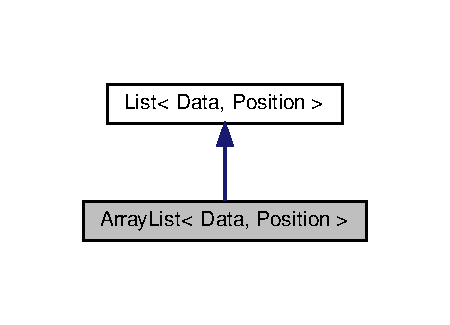
\includegraphics[width=216pt]{class_array_list__inherit__graph}
\end{center}
\end{figure}


Collaboration diagram for Array\+List$<$ Data, Position $>$\+:\nopagebreak
\begin{figure}[H]
\begin{center}
\leavevmode
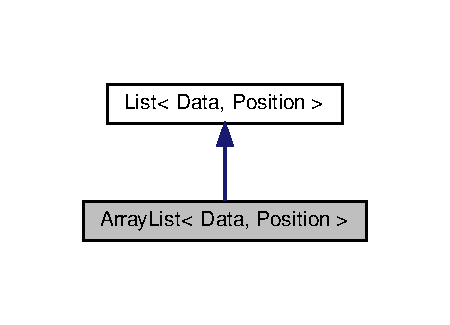
\includegraphics[width=216pt]{class_array_list__coll__graph}
\end{center}
\end{figure}
\subsection*{Public Member Functions}
\begin{DoxyCompactItemize}
\item 
\mbox{\Hypertarget{class_array_list_a51b1ac71633b2903de328170dc5b9eb9}\label{class_array_list_a51b1ac71633b2903de328170dc5b9eb9}} 
void {\bfseries resizer} ()
\item 
\mbox{\Hypertarget{class_array_list_a17e5748065133b10e0baf6a0d53d621e}\label{class_array_list_a17e5748065133b10e0baf6a0d53d621e}} 
void {\bfseries empty\+List} ()
\item 
\mbox{\Hypertarget{class_array_list_a8dd688c1bd165785e6960afe597fe81b}\label{class_array_list_a8dd688c1bd165785e6960afe597fe81b}} 
void {\bfseries reorder} (Data data, Position position)
\item 
\mbox{\Hypertarget{class_array_list_a9587a052d1433bfa89fd31e573f06c36}\label{class_array_list_a9587a052d1433bfa89fd31e573f06c36}} 
void {\bfseries reorder\+\_\+inv} (Data data, Position position)
\item 
\mbox{\Hypertarget{class_array_list_adf1a83e0c2e620909f1bed069ce30a73}\label{class_array_list_adf1a83e0c2e620909f1bed069ce30a73}} 
void {\bfseries insertt} (Data data)
\item 
\mbox{\Hypertarget{class_array_list_ab8bea1e4dc8b60b984bfd9b14008ee7d}\label{class_array_list_ab8bea1e4dc8b60b984bfd9b14008ee7d}} 
void {\bfseries insert} (Data, Position $\ast$)
\item 
\mbox{\Hypertarget{class_array_list_aa99e6236fc1a6f8d42c83d4d503f3794}\label{class_array_list_aa99e6236fc1a6f8d42c83d4d503f3794}} 
Position \& {\bfseries insert} (const Data \&d)
\item 
\mbox{\Hypertarget{class_array_list_a86044618d06ad064bdb43461f87a1d55}\label{class_array_list_a86044618d06ad064bdb43461f87a1d55}} 
void {\bfseries remove} (Position $\ast$)
\item 
\mbox{\Hypertarget{class_array_list_a1e8699311db3c7341d0cffacd54e9c7d}\label{class_array_list_a1e8699311db3c7341d0cffacd54e9c7d}} 
Data {\bfseries get\+Element} (Position $\ast$)
\item 
\mbox{\Hypertarget{class_array_list_aa5e024be6f38dc20b695a1eef27dfb0a}\label{class_array_list_aa5e024be6f38dc20b695a1eef27dfb0a}} 
Position $\ast$ {\bfseries next} (Position $\ast$)
\item 
\mbox{\Hypertarget{class_array_list_a29582f955cc0f96c98dc39e8c170d553}\label{class_array_list_a29582f955cc0f96c98dc39e8c170d553}} 
Position $\ast$ {\bfseries prev} (Position $\ast$)
\item 
\mbox{\Hypertarget{class_array_list_a31a793ebb8ab9f2ab4e58cc5bf9c4f15}\label{class_array_list_a31a793ebb8ab9f2ab4e58cc5bf9c4f15}} 
void {\bfseries insert} (Data data, Position position)
\item 
\mbox{\Hypertarget{class_array_list_af2c5f1d24667ea4ab4db08ecfc5d8e5e}\label{class_array_list_af2c5f1d24667ea4ab4db08ecfc5d8e5e}} 
void {\bfseries remove} (Data data)
\item 
\mbox{\Hypertarget{class_array_list_a91f056a60914263b1d5c97cb2c8b0b35}\label{class_array_list_a91f056a60914263b1d5c97cb2c8b0b35}} 
void {\bfseries remove} (Position position)
\item 
\mbox{\Hypertarget{class_array_list_a6a77f7f12b978b7ecd2811e00498ef8f}\label{class_array_list_a6a77f7f12b978b7ecd2811e00498ef8f}} 
Data {\bfseries get\+Element} (Position position)
\item 
\mbox{\Hypertarget{class_array_list_aa6f8a6339fed33d585a1890f9f1254e7}\label{class_array_list_aa6f8a6339fed33d585a1890f9f1254e7}} 
Position $\ast$ {\bfseries find} (Data data)
\item 
\mbox{\Hypertarget{class_array_list_a4971334b33640242e64f5e8940b96052}\label{class_array_list_a4971334b33640242e64f5e8940b96052}} 
Position $\ast$ {\bfseries next} (Position position)
\item 
\mbox{\Hypertarget{class_array_list_a6efdfdc5cf1bde019938682b83bc0e26}\label{class_array_list_a6efdfdc5cf1bde019938682b83bc0e26}} 
Position $\ast$ {\bfseries prev} (Position position)
\item 
\mbox{\Hypertarget{class_array_list_aa1e6bad9eec99411e04abb8ca52e9f58}\label{class_array_list_aa1e6bad9eec99411e04abb8ca52e9f58}} 
void {\bfseries print} ()
\end{DoxyCompactItemize}
\subsection*{Public Attributes}
\begin{DoxyCompactItemize}
\item 
\mbox{\Hypertarget{class_array_list_aad082c0109880cc13258b44f782519b2}\label{class_array_list_aad082c0109880cc13258b44f782519b2}} 
Data $\ast$ {\bfseries arreglo}
\item 
\mbox{\Hypertarget{class_array_list_adcead6da2aaf9a0df26b8a9ced623c0a}\label{class_array_list_adcead6da2aaf9a0df26b8a9ced623c0a}} 
int {\bfseries numero\+\_\+items} =0
\item 
\mbox{\Hypertarget{class_array_list_acc408eae4e59773579790c20d92762e0}\label{class_array_list_acc408eae4e59773579790c20d92762e0}} 
int {\bfseries items\+\_\+activos} =0
\end{DoxyCompactItemize}


\subsection{Detailed Description}
\subsubsection*{template$<$typename Data, typename Position$>$\newline
class Array\+List$<$ Data, Position $>$}



Definition at line 7 of file Array\+List.\+h.



The documentation for this class was generated from the following file\+:\begin{DoxyCompactItemize}
\item 
/home/jzunigame/\+Documentos/\+A\+\_\+\+Algoritmos/\+A\+\_\+\+Git/\+Laboratorios/\+Lab4 Listas/include/Array\+List.\+h\end{DoxyCompactItemize}

\hypertarget{class_list}{}\section{List$<$ Data, Position $>$ Class Template Reference}
\label{class_list}\index{List$<$ Data, Position $>$@{List$<$ Data, Position $>$}}


Inheritance diagram for List$<$ Data, Position $>$\+:\nopagebreak
\begin{figure}[H]
\begin{center}
\leavevmode
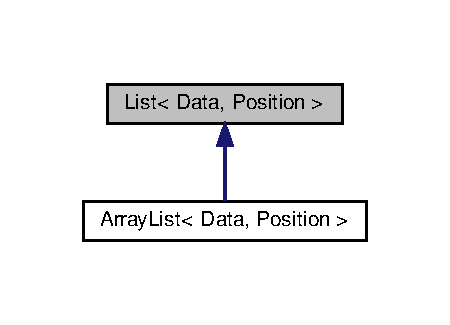
\includegraphics[width=216pt]{class_list__inherit__graph}
\end{center}
\end{figure}
\subsection*{Public Member Functions}
\begin{DoxyCompactItemize}
\item 
\mbox{\Hypertarget{class_list_a57165b01e9b6e343ec2fd429b55845f1}\label{class_list_a57165b01e9b6e343ec2fd429b55845f1}} 
{\bfseries List} (const \hyperlink{class_list}{List} \&orig)
\item 
\mbox{\Hypertarget{class_list_a65dcd9c5a33efd66cb3b7150fbc57c72}\label{class_list_a65dcd9c5a33efd66cb3b7150fbc57c72}} 
virtual void {\bfseries empty\+List} ()=0
\item 
\mbox{\Hypertarget{class_list_ab552cf8902976826d52ab13ea38929fc}\label{class_list_ab552cf8902976826d52ab13ea38929fc}} 
virtual void {\bfseries insert} (Data, Position $\ast$)=0
\item 
\mbox{\Hypertarget{class_list_a278f3ff956301318ec26d4a351373194}\label{class_list_a278f3ff956301318ec26d4a351373194}} 
virtual Position \& {\bfseries insert} (const Data \&d)=0
\item 
\mbox{\Hypertarget{class_list_a5addfe02246a4a6f719f8bac1d5bd1aa}\label{class_list_a5addfe02246a4a6f719f8bac1d5bd1aa}} 
virtual void {\bfseries remove} (Data)=0
\item 
\mbox{\Hypertarget{class_list_a501e8ae849d67cd686f0c0a3d9f7992f}\label{class_list_a501e8ae849d67cd686f0c0a3d9f7992f}} 
virtual void {\bfseries remove} (Position $\ast$)=0
\item 
\mbox{\Hypertarget{class_list_af4bd172754a3e06a3a356b389065bdc7}\label{class_list_af4bd172754a3e06a3a356b389065bdc7}} 
virtual Data {\bfseries get\+Element} (Position $\ast$)=0
\item 
\mbox{\Hypertarget{class_list_ad6cc8750b1bd313747547ce94c8fbea4}\label{class_list_ad6cc8750b1bd313747547ce94c8fbea4}} 
virtual Position $\ast$ {\bfseries find} (Data)=0
\item 
\mbox{\Hypertarget{class_list_a6e3479313c8ce725def4e36a5540ea7c}\label{class_list_a6e3479313c8ce725def4e36a5540ea7c}} 
virtual Position $\ast$ {\bfseries next} (Position $\ast$)=0
\item 
\mbox{\Hypertarget{class_list_aab5e1a4acb9997e8bb406e8fdb4eabb9}\label{class_list_aab5e1a4acb9997e8bb406e8fdb4eabb9}} 
virtual Position $\ast$ {\bfseries prev} (Position $\ast$)=0
\item 
\mbox{\Hypertarget{class_list_ab9f8e23dd4cfee4122602b3724af7812}\label{class_list_ab9f8e23dd4cfee4122602b3724af7812}} 
virtual void {\bfseries print} ()=0
\end{DoxyCompactItemize}
\subsection*{Public Attributes}
\begin{DoxyCompactItemize}
\item 
\mbox{\Hypertarget{class_list_aaedf2c01a4808437b1e02c75b591022a}\label{class_list_aaedf2c01a4808437b1e02c75b591022a}} 
int {\bfseries items} = 0
\end{DoxyCompactItemize}


\subsection{Detailed Description}
\subsubsection*{template$<$typename Data, typename Position$>$\newline
class List$<$ Data, Position $>$}



Definition at line 8 of file List.\+h.



The documentation for this class was generated from the following file\+:\begin{DoxyCompactItemize}
\item 
/home/jzunigame/\+Documentos/\+A\+\_\+\+Algoritmos/\+A\+\_\+\+Git/\+Laboratorios/\+Lab4 Listas/include/List.\+h\end{DoxyCompactItemize}

\hypertarget{class_simple_position}{}\section{Simple\+Position$<$ Dato $>$ Class Template Reference}
\label{class_simple_position}\index{Simple\+Position$<$ Dato $>$@{Simple\+Position$<$ Dato $>$}}
\subsection*{Public Member Functions}
\begin{DoxyCompactItemize}
\item 
\mbox{\Hypertarget{class_simple_position_a6b6e102942c3cf1797735255897402b5}\label{class_simple_position_a6b6e102942c3cf1797735255897402b5}} 
{\bfseries Simple\+Position} (Dato $\ast$valor)
\end{DoxyCompactItemize}
\subsection*{Public Attributes}
\begin{DoxyCompactItemize}
\item 
\mbox{\Hypertarget{class_simple_position_a65bb8d8c8a3011fb28ea1a324c7910dc}\label{class_simple_position_a65bb8d8c8a3011fb28ea1a324c7910dc}} 
\hyperlink{class_simple_position}{Simple\+Position}$<$ Dato $>$ $\ast$ {\bfseries siguiente} = 0x0
\item 
\mbox{\Hypertarget{class_simple_position_adfc8434ef460d5c20d71494ad6a48c52}\label{class_simple_position_adfc8434ef460d5c20d71494ad6a48c52}} 
Dato $\ast$ {\bfseries valor}
\end{DoxyCompactItemize}


\subsection{Detailed Description}
\subsubsection*{template$<$typename Dato$>$\newline
class Simple\+Position$<$ Dato $>$}



Definition at line 8 of file Simple\+Position.\+h.



The documentation for this class was generated from the following file\+:\begin{DoxyCompactItemize}
\item 
/home/jzunigame/\+Documentos/\+A\+\_\+\+Algoritmos/\+A\+\_\+\+Git/\+Laboratorios/\+Lab4 Listas/include/Simple\+Position.\+h\end{DoxyCompactItemize}

\hypertarget{class_single_linked_list}{}\section{Single\+Linked\+List$<$ Element, Single\+Position $>$ Class Template Reference}
\label{class_single_linked_list}\index{Single\+Linked\+List$<$ Element, Single\+Position $>$@{Single\+Linked\+List$<$ Element, Single\+Position $>$}}


Collaboration diagram for Single\+Linked\+List$<$ Element, Single\+Position $>$\+:
\nopagebreak
\begin{figure}[H]
\begin{center}
\leavevmode
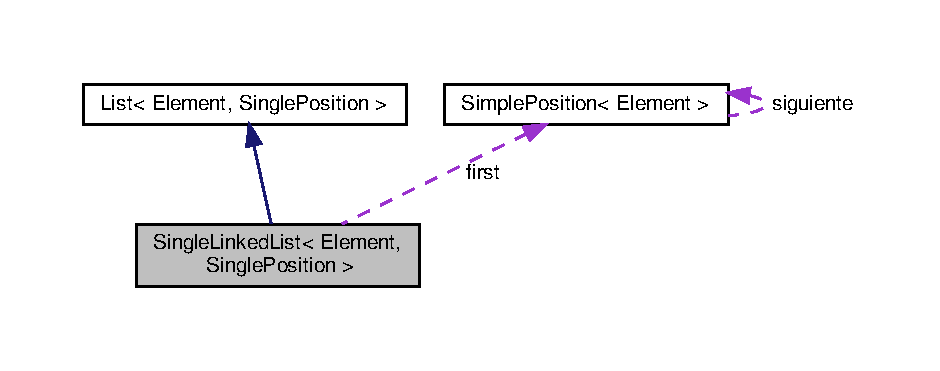
\includegraphics[width=277pt]{class_single_linked_list__coll__graph}
\end{center}
\end{figure}
\subsection*{Public Member Functions}
\begin{DoxyCompactItemize}
\item 
\mbox{\Hypertarget{class_single_linked_list_aa94809f2f418d8ae0800c07ad2d3ed94}\label{class_single_linked_list_aa94809f2f418d8ae0800c07ad2d3ed94}} 
Single\+Position \& {\bfseries insert} (const \hyperlink{class_element}{Element} \&dato)
\item 
\mbox{\Hypertarget{class_single_linked_list_a22c895b2d3effcce5983b991a380027b}\label{class_single_linked_list_a22c895b2d3effcce5983b991a380027b}} 
\hyperlink{class_element}{Element} $\ast$ {\bfseries get\+Direccion} (int elemento)
\item 
\mbox{\Hypertarget{class_single_linked_list_a64d9f3e1bad3eec787d2bcc7255c1311}\label{class_single_linked_list_a64d9f3e1bad3eec787d2bcc7255c1311}} 
void \hyperlink{class_single_linked_list_a64d9f3e1bad3eec787d2bcc7255c1311}{print} ()
\begin{DoxyCompactList}\small\item\em Funcion que imprime los datos de la lista. \end{DoxyCompactList}\item 
\mbox{\Hypertarget{class_single_linked_list_a09b8d66c2be112326210373514f32cd7}\label{class_single_linked_list_a09b8d66c2be112326210373514f32cd7}} 
Single\+Position $\ast$ {\bfseries devolver\+Posicion} (int item)
\item 
\mbox{\Hypertarget{class_single_linked_list_aebc417269f785f2f8d3689403e7a6524}\label{class_single_linked_list_aebc417269f785f2f8d3689403e7a6524}} 
bool {\bfseries verificar} (\hyperlink{class_class_node}{Class\+Node} $\ast$origen, \hyperlink{class_class_node}{Class\+Node} $\ast$destino)
\item 
\mbox{\Hypertarget{class_single_linked_list_a2ed18090fd23eba38a668e40e0bca2c4}\label{class_single_linked_list_a2ed18090fd23eba38a668e40e0bca2c4}} 
Single\+Position $\ast$ {\bfseries devolver\+Posicion\+Desde\+Valor} (int valor)
\item 
\mbox{\Hypertarget{class_single_linked_list_aa94809f2f418d8ae0800c07ad2d3ed94}\label{class_single_linked_list_aa94809f2f418d8ae0800c07ad2d3ed94}} 
Single\+Position \& {\bfseries insert} (const \hyperlink{class_element}{Element} \&dato)
\item 
\mbox{\Hypertarget{class_single_linked_list_a22c895b2d3effcce5983b991a380027b}\label{class_single_linked_list_a22c895b2d3effcce5983b991a380027b}} 
\hyperlink{class_element}{Element} $\ast$ {\bfseries get\+Direccion} (int elemento)
\item 
\mbox{\Hypertarget{class_single_linked_list_a64d9f3e1bad3eec787d2bcc7255c1311}\label{class_single_linked_list_a64d9f3e1bad3eec787d2bcc7255c1311}} 
void \hyperlink{class_single_linked_list_a64d9f3e1bad3eec787d2bcc7255c1311}{print} ()
\begin{DoxyCompactList}\small\item\em Funcion que imprime los datos de la lista. \end{DoxyCompactList}\item 
\mbox{\Hypertarget{class_single_linked_list_a09b8d66c2be112326210373514f32cd7}\label{class_single_linked_list_a09b8d66c2be112326210373514f32cd7}} 
Single\+Position $\ast$ {\bfseries devolver\+Posicion} (int item)
\item 
\mbox{\Hypertarget{class_single_linked_list_aebc417269f785f2f8d3689403e7a6524}\label{class_single_linked_list_aebc417269f785f2f8d3689403e7a6524}} 
bool {\bfseries verificar} (\hyperlink{class_class_node}{Class\+Node} $\ast$origen, \hyperlink{class_class_node}{Class\+Node} $\ast$destino)
\item 
\mbox{\Hypertarget{class_single_linked_list_a2ed18090fd23eba38a668e40e0bca2c4}\label{class_single_linked_list_a2ed18090fd23eba38a668e40e0bca2c4}} 
Single\+Position $\ast$ {\bfseries devolver\+Posicion\+Desde\+Valor} (int valor)
\end{DoxyCompactItemize}
\subsection*{Public Attributes}
\begin{DoxyCompactItemize}
\item 
\mbox{\Hypertarget{class_single_linked_list_a870bf08579b5a9cb4d570b57cbcdc826}\label{class_single_linked_list_a870bf08579b5a9cb4d570b57cbcdc826}} 
\hyperlink{class_simple_position}{Simple\+Position}$<$ \hyperlink{class_element}{Element} $>$ $\ast$ {\bfseries first}
\item 
\mbox{\Hypertarget{class_single_linked_list_a8449fa747af940f9d1c9c6e8758539b8}\label{class_single_linked_list_a8449fa747af940f9d1c9c6e8758539b8}} 
int {\bfseries items} =0
\end{DoxyCompactItemize}


\subsection{Detailed Description}
\subsubsection*{template$<$typename Element, typename Single\+Position$>$\newline
class Single\+Linked\+List$<$ Element, Single\+Position $>$}



Definition at line 9 of file Single\+Linked\+List.\+h.



The documentation for this class was generated from the following file\+:\begin{DoxyCompactItemize}
\item 
Algoritmos\+De\+Terceros/include/\+Listas/Single\+Linked\+List.\+h\end{DoxyCompactItemize}

%--- End generated contents ---

% Index
\backmatter
\newpage
\phantomsection
\clearemptydoublepage
\addcontentsline{toc}{chapter}{Index}
\printindex

\end{document}
